Many ideas have been shaped in order to make websites more dynamic and avoid breaking the site when loading a new \gls{html} file from the server. One pattern that solves this problem efficiently is the \gls{mvu} application pattern.
To solve the problem of showing diverged information in an \gls{html} document, the JavaScript language is needed, as there is no native and complex enough support for \gls{html} or \gls{css} to force the browser to show this new information. JavaScript on the other hand can directly inject into the \gls{dom}, by having complete access to every \gls{html} node element in the rendered \gls{dom}.
JavaScript can select a node element by \texttt{ID} and change its displayed value, forcing the browser to rerender the \gls{dom} on that node. Figure \ref{fig:button_browser} shows a minimal example, where JavaScript is used to alter the rendered \gls{html}.

\begin{figure}
    \centering
    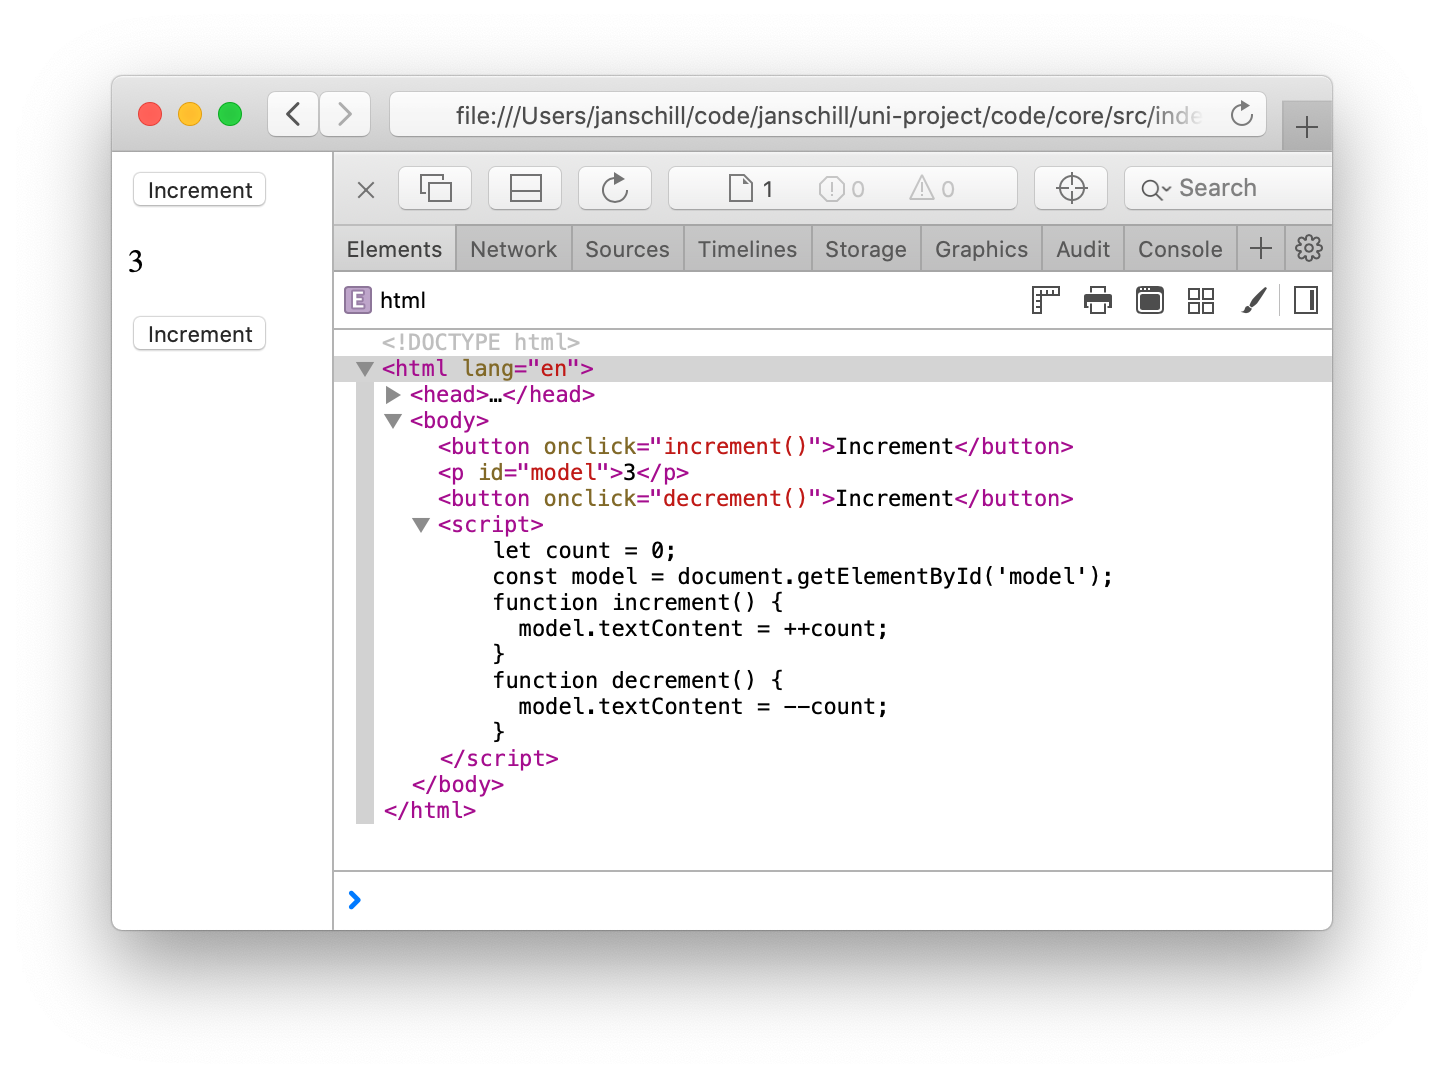
\includegraphics[width=0.8\textwidth]{images/button-browser.png}
    \caption{Simple button counter example}
    \label{fig:button_browser}
\end{figure}

This way of updating content on the document directly has been evolved over the years and is heavily used to build any sized modern websites. With the help of frameworks like React\footnote{\url{https://reactjs.org/}}, a JavaScript framework developed by Facebook or Elm\footnote{\url{https://elm-lang.org/}}, a framework utilizing its own functional language, it has become easier to go from a small button example to a fully working componentized website.
The Elm framework uses the \gls{mvu} application pattern to realize the idea of dynamically updating the \gls{dom}.

The basic functionality how Elm uses it, is as follows. The framework generates \gls{html} that can be viewed by a client. This client can then interact with the \gls{html} by clicking a button for example. This produces a \texttt{Msg (Message)}, which is send to Elm, that generates another \gls{html} document. This cycle is what is referred to as the \gls{mvu} cycle.
In the Elm program three parts play a crucial role: The Model, View and Update.

When a message of type \texttt{Msg} is produced, the update function is being called, which takes the message and the current state of the model and returns an updated model. The view function, which is responsible of generating the \gls{html} that can be viewed by the browser, is then called automatically, rendering the \gls{html} with the updated model.

\begin{lstlisting}[columns=fullflexible, label={view_model}, language=Other, caption={View, update and model and their types}]
view : Model -> Html Msg
update : Msg -> Model -> Model
\end{lstlisting}

\paragraph{How does Elm optimize the view rendering?}
Oftentimes when a new view is generated and needs to be re-rendered, it is not necessary for the whole document to be switched out, but rather only the \gls{dom} node that experienced change. Forcing the browser to generate new \gls{dom} nodes is computational expensive work.
For this most frameworks use a \gls{vdom}, which resembles the complete active \gls{dom} in memory in a convenient data structure. The \gls{vdom} is generated with the updated model and compared against the current active \gls{vdom}, finding the parts that need updating. This part is called \textit{diffing} and it is done by iterating over both representations of the \gls{dom} and comparing each individual node. This \textit{diffing} then generates a data structure that keeps track of all changes. A \textit{patch} function takes the old view and the data structure holding the changes, which then updates all occurrences of change in the view.

All the \textit{diffing} and \textit{patching} against the \gls{dom} tree seems to be still computational expensive, as in the end, only the following code snippet is actually needed for the button example to work:

\begin{lstlisting}[columns=fullflexible, label={button_increment}, language=Other, caption={Reduced example to show only the incrementing}]
<html>
  <button onclick=increment()>Increment</button>
  <p id="model">0</p>
</html>
<script>
  let count = 0;
  const model = document.getElementById('model');
  function increment() {
    model.textContent = ++count;
  }
</script>
\end{lstlisting}

\paragraph{How does JaLi optimize the view rendering even further?} This paper will outline all the needed parts to use partial evaluation, symbolic execution and constant folding to optimize the view rendering. It will be shown on the small button example how the compiler of the JaLi language can reduce all the previously mentioned parts that are computational expensive, by applying the optimizations.
Due to time restrictions and the sheer complexity of the project it was not able to implement the full working compiler optimizations, but enough to demonstrate reduction on certain programs. A compiler that transforms a full program to a \gls{html} and JavaScript website that can run in the browser is also not implemented---this will be simulated by manual coding the JavaScript parts. Nevertheless, the theory has been established and it will be shown on small examples to illustrate the idea.

In the following chapter the functional language that was developed for this project will be explained. The next chapter describes partial evaluation and how reduction is carried out on the JaLi language. Next the implementation of the \gls{mvu} in the JaLi language is shown, and lastly the button example will be used to show how it can reduced into functioning \gls{html} and JavaScript that avoids the \gls{mvu} cycle and the \gls{vdom} diffing.
